\documentclass[12pt,a4paper]{NirmaThesis}


\AtBeginDocument{\renewcommand{\bibname}{References}}
%\DeclareGraphicsExtensions{.pdf,.jpeg,.png}

%Define all the packages needed in your report here
\usepackage[pdftex]{graphicx}
\usepackage{hyperref}
\usepackage{caption}
\usepackage{subcaption}
\usepackage[top=1in, bottom=1in, left=1in, right=1in]{geometry}
\usepackage[compact]{titlesec}
\usepackage{setspace}
\usepackage{amsmath}
\usepackage{placeins}


\renewcommand{\baselinestretch}{1.5}
\newcommand{\HRule}{\rule{\linewidth}{0.8mm}}
\renewcommand{\chaptermark}[1]{%
\markboth{\thechapter.\ #1}{}}
\hypersetup{colorlinks, filecolor=black, linkcolor=black, pdftex}



\begin{document}
\renewcommand{\thepage}{\roman{page}}
%Prepare your coverpages in coverpages.tex file and include it here.
% TITLE PAGE

\thispagestyle{empty}
\begin{center}
{\huge Title of the Project }\vspace{.05in}\\

\vspace{4cm}

Submitted By\\
%\vspace{0.2cm}
{\large \bf Student Name} \\
{\bf Roll No} \\
\vspace{10cm}



\begin{figure}[h]
\begin{center}
  % Requires \usepackage{graphicx}
  
\includegraphics [scale=0.7]{NU_IT_Color_Max.png}\\
\end{center}
\end{figure}

\vspace{-0.5cm}
{\bf DEPARTMENT OF COMPUTER SCIENCE AND ENGINEERING}\\
{\bf INSTITUTE OF TECHNOLOGY}\\
{\bf NIRMA UNIVERSITY}\\
{\bf AHMEDABAD-382481}\\
{\bf December 2014}
\end{center}

% ------------------------------------------------------------------------------------------------
\newpage
\thispagestyle{empty}
\begin{center}

\HRule \\
{\huge Title of the Project}\vspace{.05in}\\
\HRule

\vspace{1cm}
{\large \bf Major Project}\\
\vspace{0.6cm}

{
Submitted in partial fulfillment of the requirements\\
\vspace{0.3cm}
for the degree of\\
\vspace{0.3cm}
Master of Technology in Computer Science and Engineering\\
}
\vspace{0.8cm} Submitted By\\
{\large \bf Student Name} \\
{\bf (Roll No.)} \\
\vspace{0.8cm}

Guided By \\
{{\large\bf {Guide Name}}} \\
\vspace{4.5cm}
\begin{figure}[h]
\begin{center}
  
\includegraphics [scale=0.7]{NU_IT_Color_Max.png}\\
\end{center}
\end{figure}

\vspace{-0.5cm}
{\bf DEPARTMENT OF COMPUTER SCIENCE AND ENGINEERING}\\
{\bf INSTITUTE OF TECHNOLOGY}\\
{\bf NIRMA UNIVERSITY}\\
{\bf AHMEDABAD-382481}\\
{\bf December 2014}
\end{center}


%------------------------------------------------------------------------------------------------------------------
\newpage
\vspace{4cm}
\addcontentsline{toc}{chapter}{Certificate}\index{Certificate}
\begin{center}
{\Large \bf Certificate}\\
\end{center}
\vspace{10pt}

\noindent This is to certify that the major project entitled
 \textbf{"Tile of the Project"} submitted by \textbf{Student Name (Roll No: 13MCECXX)}, towards the partial fulfillment of the requirements for the award of degree of Master of Technology in Computer Science and Engineering of Nirma University, Ahmedabad, is the record of work carried out by him under my supervision and guidance. In my opinion, the submitted work has reached a level required for being accepted for examination. The results embodied in this project, to the best of my knowledge, haven't been submitted to any other university or institution for award of any degree or diploma. \\
\vspace{2cm} \\
\noindent


\vspace{2cm} \noindent
\begin{tabular}{ l p{3.1cm}lp{4cm}l }
Prof. K. P. Agrawal & \hspace{0.3cm} & Prof. Vijay Ukani\\
Guide \& Associate Professor, & & Associate Professor, \\
CSE Department, & & Coordinator M.Tech - CSE\\
Institute of Technology, & & Institute of Technology,\\
Nirma University, Ahmedabad. & & Nirma University, Ahmedabad\\
\end{tabular} \\



\vspace{2cm} \noindent
\begin{tabular}{ l p{3.1cm}lp{4cm}l }
Dr. Sanjay Garg & \hspace{0.3cm} & Dr K Kotecha\\
Professor and Head, & & Director, \\
CSE Department, & & Institute of Technology,\\
Institute of Technology, & & Nirma University, Ahmedabad\\
Nirma University, Ahmedabad. & & \\
\end{tabular} \\



% -----------------------------------------------------------------------------------------------------------------
\newpage
\vspace{4cm}
\addcontentsline{toc}{chapter}{Statement of Originality}\index{Statement of Originality}
\begin{center}
%{\Large \bf Annexure VI}\\
{\Large \bf Statement of Originality}\\
\end{center}
\vspace{-0.6cm}
---------------------------------------------------------------------------------------------------------------------\\
\noindent I, \textbf{Student Name}, Roll. No. \textbf{13MCECXX}, give undertaking that the Major Project entitled "\textbf{Title of the Project}" submitted by me, towards the partial fulfillment of the requirements for the degree of Master of Technology in \textbf{Computer Science \& Engineering} of Institute of Technology, Nirma University, Ahmedabad, contains no material that has been awarded for any degree or diploma in any university or school in any territory to the best of my knowledge. It is the original work carried out by me and I give assurance that no attempt of plagiarism has been made. It contains no material that is previously published or written, except where reference has been made. I understand that in the event of any similarity found subsequently with any published work or any dissertation work elsewhere; it will result in severe disciplinary action.



\vspace{2cm}
-----------------------\\
Signature of Student\\
Date:\\
Place:\\
\begin{flushright}
Endorsed by \\
Guide Name \\
(Signature of Guide)
\end{flushright}



%------------------------------------------------------------------------------------------------------------------------
%ACKNOLEDGEMENT PAGE
\newpage
\addcontentsline{toc}{chapter}{Acknowledgements}\index{Acknowledgements}
\begin{center}
{\Large \bf Acknowledgements}\\
\end{center}
\vspace{10pt}
It gives me immense pleasure in expressing thanks and profound gratitude to \textbf{Prof. X. Y. Abcedef}, Associate Professor, Computer Science Department, Institute of Technology, Nirma University, Ahmedabad for his valuable guidance and continual encouragement throughout this work. The appreciation and continual support he has imparted has been a great motivation to me in reaching a higher goal. His guidance has triggered and nourished my intellectual maturity that I will benefit from, for a long time to come.\\

It gives me an immense pleasure to thank \textbf{Dr. Sanjay Garg}, Hon'ble Head of Computer Science and Engineering Department, Institute of Technology, Nirma University, Ahmedabad for his kind support and providing basic infrastructure and healthy research environment.\\

A special thank you is expressed wholeheartedly to \textbf{Dr K Kotecha}, Hon'ble Director, Institute of Technology, Nirma University, Ahmedabad for the unmentionable motivation he has extended throughout course of this work.\\

I would also thank the Institution, all faculty members of Computer Engineering Department, Nirma University, Ahmedabad for their special attention and suggestions towards the project work.

See that you acknowledge each one who have helped you in the project directly or indirectly.
\\



\begin{flushright}
\textbf{- Student Name}\\ \textbf{13MCECXX}
\end{flushright}

% -----------------------------------------------------------------------------------------------------------------
% ABSTRACT
\newpage
\addcontentsline{toc}{chapter}{Abstract}\index{Abstract}
\begin{center}
{\Large \bf Abstract}\\
\end{center}
\vspace{10pt}

Clustering aggregation problem is a kind of formal description for clustering ensemble problem and technologies for the solving of clustering aggregation problem can be used to construct clustering division with better clustering performance when the clustering performances of each original clustering division are fluctuant or weak. In this paper, an approach based on genetic algorithm for clustering aggregation problem, named as GeneticCA, is presented To estimate the clustering performance of a clustering division, clustering precision is defined and features of clustering precision are discussed In our experiments about clustering performances of GeneticCA for document clustering, hamming neural network is used to construct clustering divisions with fluctuant and weak clustering performances. Experimental results show that the clustering performance of clustering division constructed by GeneticCA is better than clustering performance of original clustering divisions with clustering precision as criterion.\\




%-----------------------------------------------------------------------------------------------------------------
% ADDING CONVENTIONS IS OPTIONAL. If you wish to remove it, delete or comment it from here.
%-----------------------------------------------------------------------------------------------------------------

%\newpage
%\addcontentsline{toc}{chapter}{Conventions}\index{Conventions}
%\begin{Huge}
%Conventions\\
%\end{Huge}
%
%\vspace{50px}
%\begin{huge}
%Typesetting\\
%\end{huge}
%
%\begin{Large}
%This thesis is typeset using Latex software.\\
%Font used in this thesis are of Times new roman family.\\
%\end{Large}
%
%\vspace{20px}
%\begin{huge}
%Referencing\\
%\end{huge}
%--------------------------------------------------------------------------------------------------------------------\\
%\begin{Large}
%Referencing and citation style adopted in this thesis is ieee transaction(ieeetr).\\
%For electronic references, Last publication date is shown here.\\
%\end{Large}
%
%\vspace{20px}
%\begin{huge}
%Spelling \\
%\end{huge}
%--------------------------------------------------------------------------------------------------------------------\\
%\begin{Large}
%The Unites States English Spelling is adopted here.\\
%\end{Large}
%
%\vspace{20px}
%\begin{huge}
%Units \\
%\end{huge}
%--------------------------------------------------------------------------------------------------------------------\\
%\begin{Large}
%The Units used in This thesis are based in the International System of Units(SI Units), unless specified.
%\end{Large}



%-----------------------------------------------------------------------------------------------------------------
% Keep deleting/commenting till here in order to remove conventions.
%-----------------------------------------------------------------------------------------------------------------


\newpage
\addcontentsline{toc}{chapter}{Abbreviations}\index{Abbreviations}
\begin{Huge}
Abbreviations\\
\end{Huge}

%\begin{Large}
\begin{tabular}{ l p{0.5cm} l }
%for every term, a record is needed with following structure
% \textbf{TERM} && Description
\textbf{DBSCAN} & & Density-based spatial clustering of applications with noise. \\
\textbf{QGIS} & & Quantum geographic information systems.\\
\textbf{LEACH} & & Low Energy Adaptive Clustering Hierarchy.\\
\textbf{FCM} & & Fuzzy C-Means\\
\end{tabular}
%\end{Large}


--------------------------------------------------------------------------------------------------------------------\\



\begin{singlespace}
%This command inserts Table of Contents in the report
\tableofcontents

%This command inserts List of Figures in the report
\listoffigures 
\addcontentsline{toc}{chapter}{List of Figures}


%This command inserts List of Tables in the report
\listoftables 
\addcontentsline{toc}{chapter}{List of Tables}
\end{singlespace}


%Actual arabic page number starts here.
\pagenumbering{arabic}

%Include all chapter.tex files here. It is avisable to create separate .tex file for each chapter and include it here. However you can always type your contents here directly.

\chapter{Introduction}

\section{Knowledge Discovery Process}

Data mining is the process of discovering interesting patterns and
knowledge from large amounts of data. The data sources can include databases, data
warehouses, theWeb, other information repositories, or data that are streamed into the
system dynamically.\\

Knowledge Discovery Process Steps \cite{k1} :-
\begin{itemize}

\item {Cleaning the Data.}
\item{Integrate Data.}
\item{Select Data .}
\item{Transformation of Data.}
\item{Data mining.}
\item{Pattern finding.}

\end{itemize}


\chapter{Literature Survey}

\section{Techniques  :-} 

Although a very rudimentary learning scheme, 1R does accommodate both missing
values and numeric attributes. It deals with these in simple but effective ways.
Missing is treated as just another attribute value so that, for example, if the weather
data had contained missing values for the outlook attribute, a rule set formed on
outlook would specify four possible class values, one for each of sunny, overcast,
and rainy, and a fourth for missing.\\



{\bf Techniques shown in table:\cite{k3} }


\begin{table}[h]
\centering
\begin{tabular}{|l|l|l|l|l|}
\hline
\multicolumn{1}{|c|}{\textbf{head1}} & \multicolumn{1}{c|}{\textbf{head2}} & \multicolumn{1}{c|}{\textbf{head3}} & \multicolumn{1}{c|}{\textbf{head4}} & \multicolumn{1}{c|}{\textbf{head5}} \\ \hline
a & b & c & d & e \\ \hline
l & m & n & o & t \\ \hline
v & w & x & y & z \\ \hline
\end{tabular}
\caption{My caption}
\label{my-label}
\end{table}


Sample Table shown in table \ref{my-label} .

The diverse density is defined as the probability of the class labels of the bags
in the training data, computed based on this probabilistic model. It is maximized
when the reference point is located in an area where positive bags overlap and no
negative bags are present, just as for the two geometric methods discussed previously.
A numerical optimization routine such as gradient ascent can be used to find
the reference point that maximizes the diverse-density measure. In addition to the
location of the reference point, implementations of diverse density also optimize the
scale of the distance function in each dimension because generally not all attributes
are equally important. This can improve predictive performance significantly.\\



\chapter{Demo Chapter}

\section{Sample Comparison}

\subsection{Comparison Graph:}



figure \ref{fig:comparison-1 graph} and \ref{fig:comparison-2 graph} shows comparison:\cite{k3} \cite{k4}

\begin{figure}[h!]
					\centering

					\begin{minipage}[b]{0.45\linewidth}
					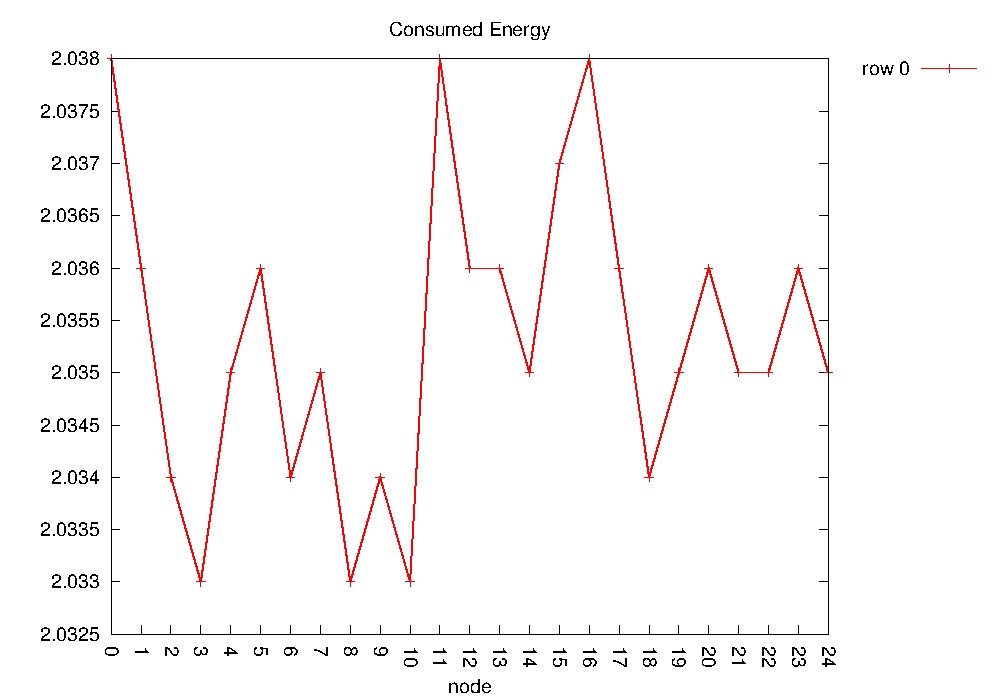
\includegraphics[scale=0.4]{demo1}
					\caption{comparison-1 graph }	
					\label{fig:comparison-1 graph}				
					\end{minipage}
					\quad
					\begin{minipage}[b]{0.45\linewidth}
					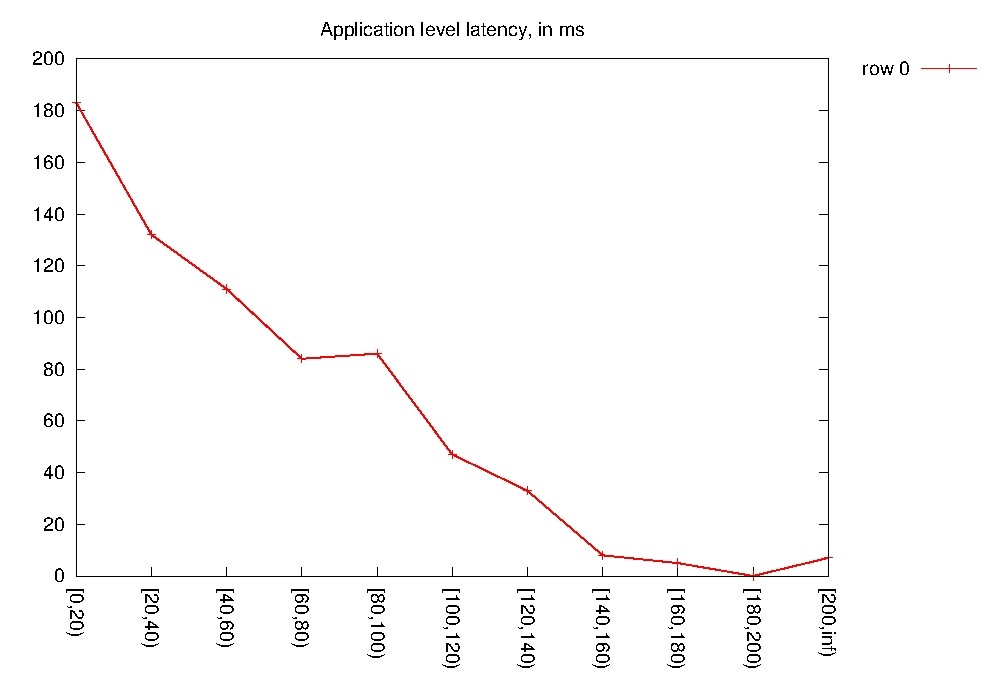
\includegraphics[scale=0.4]{demo2}
					\caption{comparison-2 graph}
					\label{fig:comparison-2 graph}
					\end{minipage}
               
      
 \end{figure}

\chapter{New Demo Chapter}

\section{Sample Experiment}

				\begin{figure}[h!]
					\centering
					\begin{minipage}[b]{0.80\linewidth}
               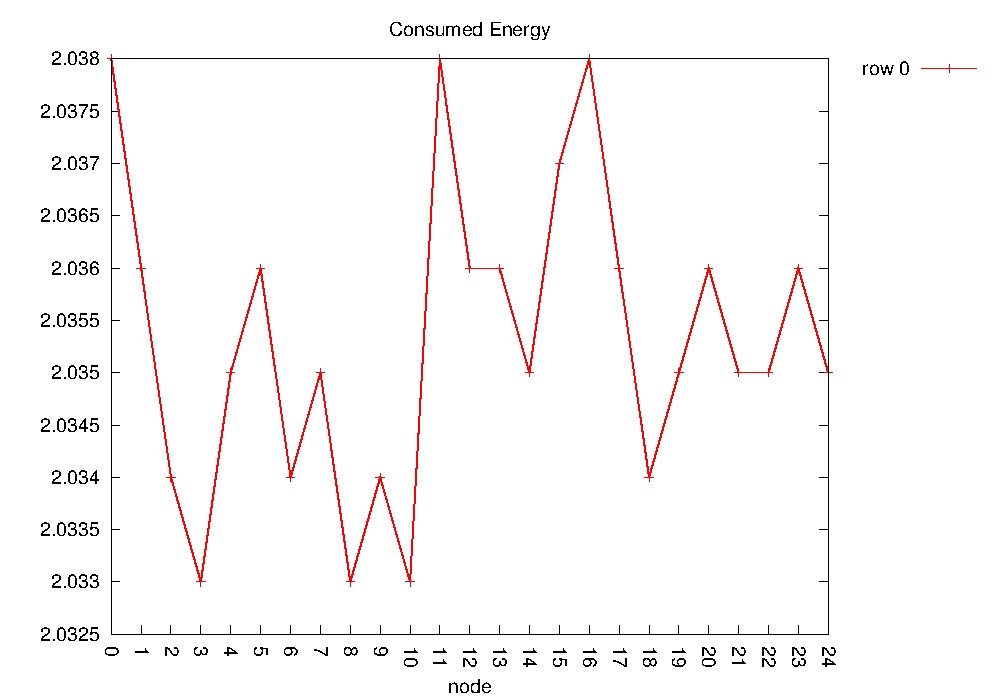
\includegraphics[scale=0.6]{demo1}
                \caption{demo figure 1}						
                \label{fig:demo1}
                \end{minipage}
                \end{figure}
                
                
     \newpage
    
 \section{Equation}    
  
  
{\bf Example Equations \cite{k3} }  
     
     \begin{equation}
  \label{eq:Continued_fractions}
  x = a_0 + \cfrac{1}{a_1
          + \cfrac{1}{a_2
          + \cfrac{1}{a_3 + \cfrac{1}{a_4} } } }
\end{equation}


\begin{equation}
  \label{eq:Multiplication}
\frac{
    \begin{array}[b]{r}
      \left( x_1 x_2 \right)\\
      \times \left( x'_1 x'_2 \right)
    \end{array}
  }{
    \left( y_1y_2y_3y_4 \right)
  }
\end{equation}


Equation \ref{eq:Continued_fractions} is a Continued fractions.\\
Equation \ref{eq:Multiplication} is Multiplication of two numbers.

%whaterver you put in $....$ will be displayed as math

$\sqrt{\frac{a}{b}}$ %this is comment, you can not cite this equation


$\sqrt[n]{1+x+x^2+x^3+\ldots}$           

\chapter{New Sample Chapter}

\section{Sample Algorithm:}

				\begin{figure}[h!]
					\centering
					\begin{minipage}[b]{0.80\linewidth}
               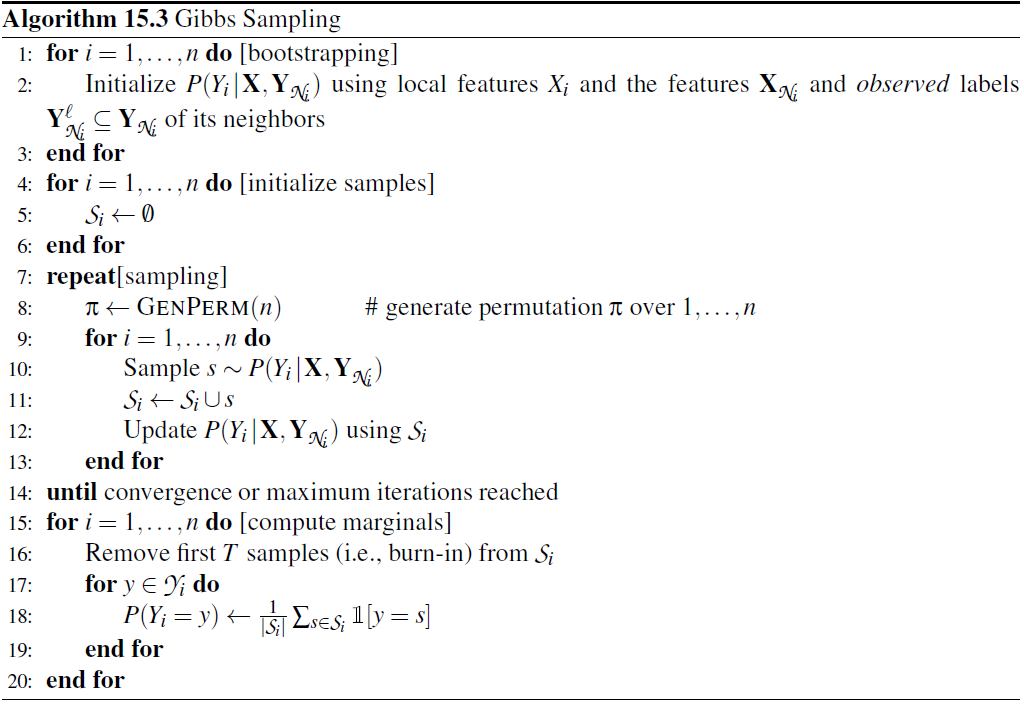
\includegraphics[scale=0.6]{sample_algo}
                \caption{Sample Algorithm}						
                \label{fig:algo1}
                \end{minipage}
                \end{figure}
                
    
 Sample Algorithm shown in figure \ref{fig:algo1} Gibbs Sampling.

\newpage

%This command sets the bibliography style and conntect your bib database file to your latex source report file.
\bibliographystyle{ieeetr}
\addcontentsline{toc}{chapter}{References}
\bibliography{mybib}

\end{document}
